We choose to train our patch model from scratch as opposed to improving the model in Q2.1, owing experience of starting from scratch in Q2.1.
Our results (see Figure \ref{fig:Q2_2}) were poor compared to the background model, which we attribute to multiple factors.
\begin{figure}[h!]
  \begin{center}
  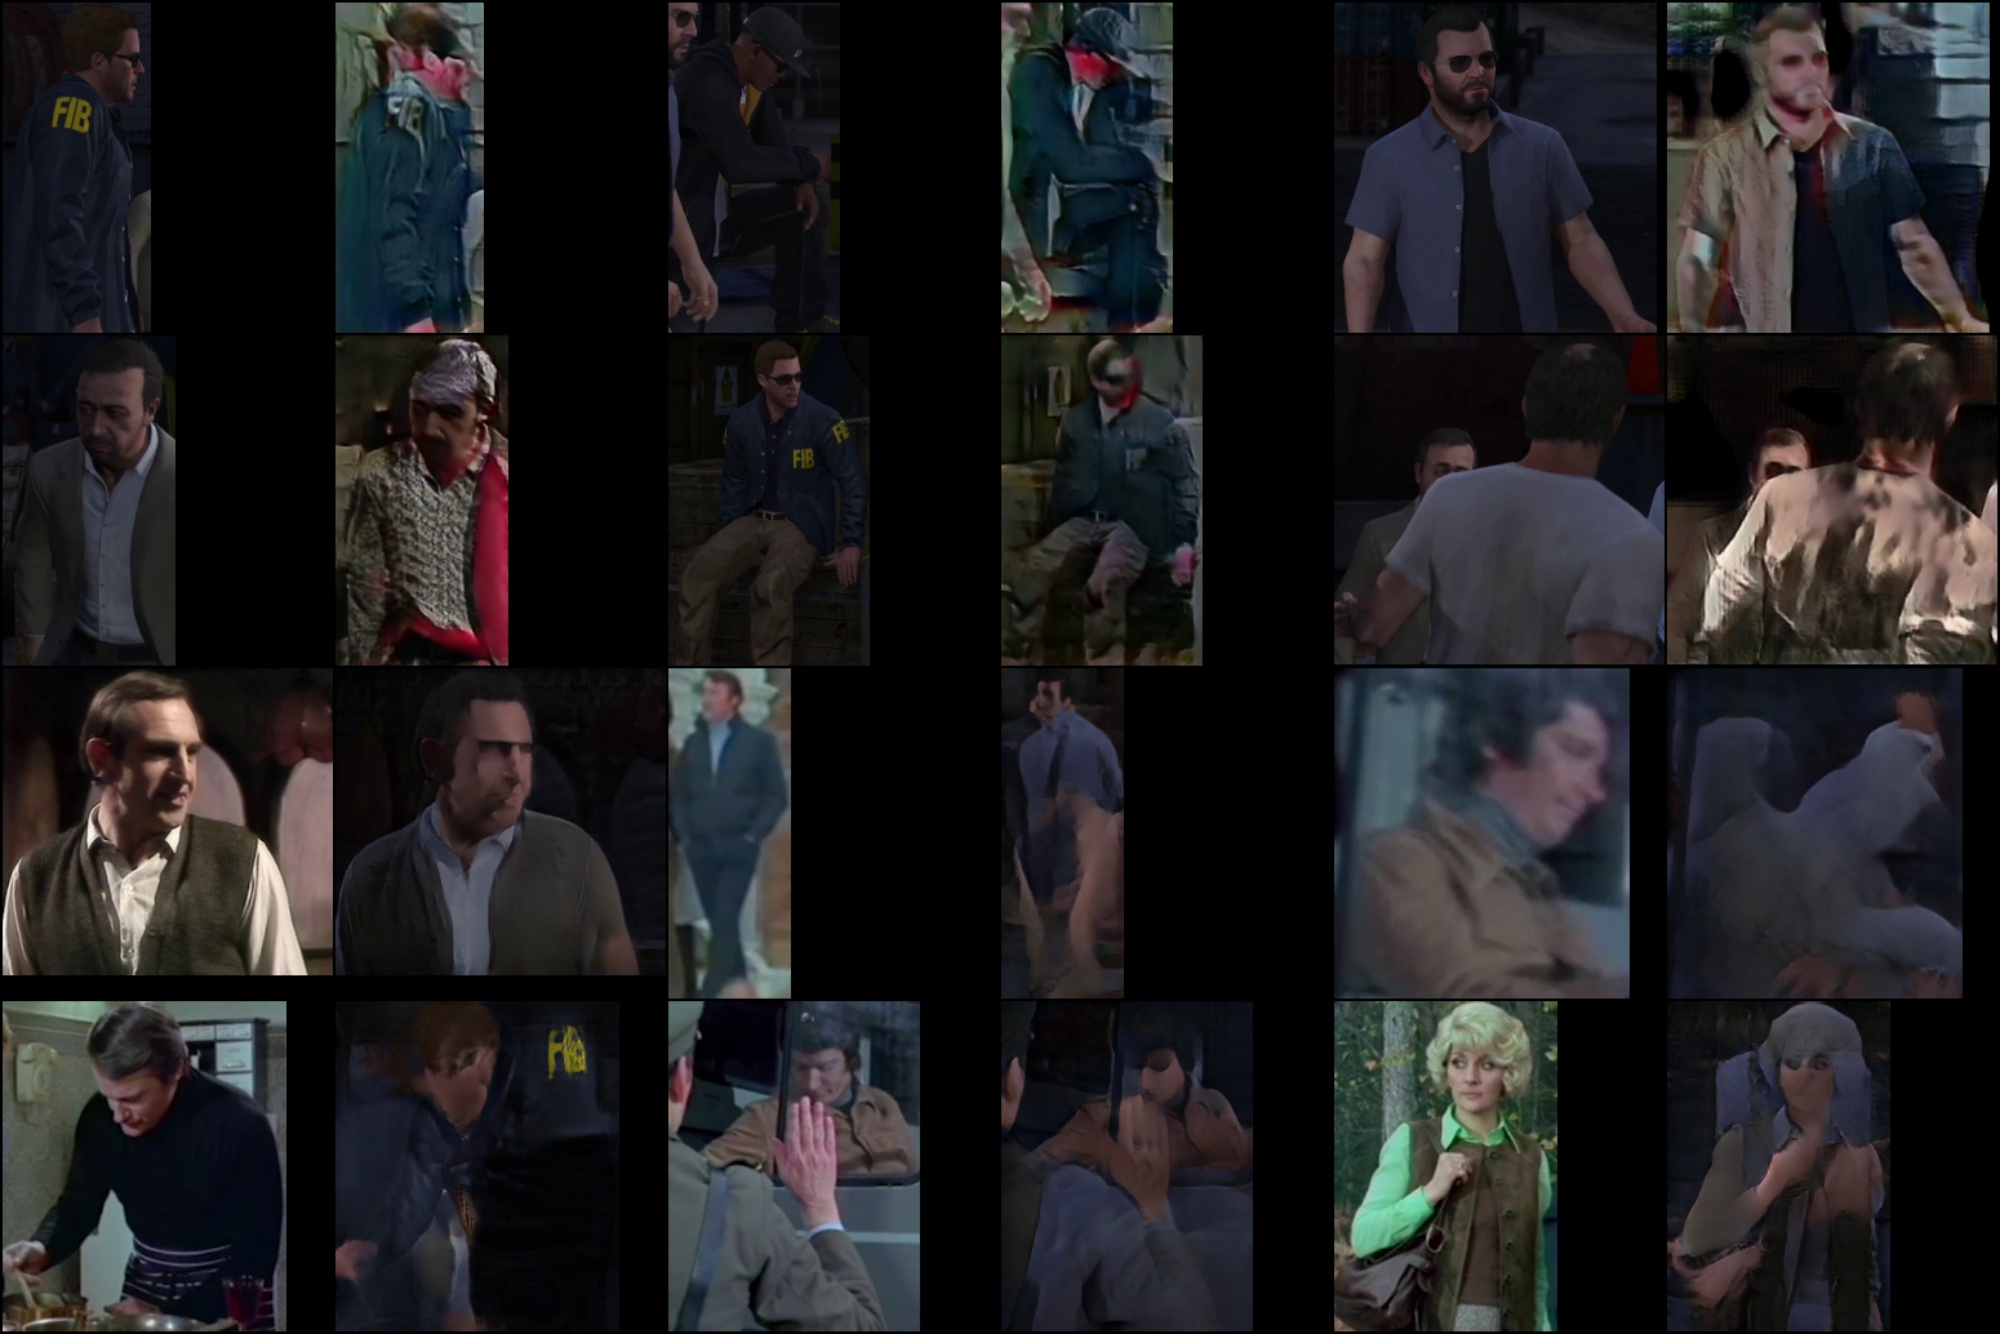
\includegraphics[scale=0.2]{Q2_2_pad.jpg}
    \caption{Q2.2 sample of patch frames (left) and style transfer into other domain (right).}
    \label{fig:Q2_2}
  \end{center}
  \end{figure}

Firstly, our training time was approx $25\%$ of that of the background model.
Also, we didn't use any augmentations, we found that augmentations proved vital in Q2.1, so not using them was a significant disadvantage.

We did however learn that maintaining aspect ratio to standardize the size of patches was the best method, as mentioned in Q1.4.
There are many places for improvement, many of which we apply to Q2.3.
It would also be interesting to see if adapting the background would be a better technique than training from scratch, as our final background models proved remarkably effective.
